%%% Henrik Sopart, 836188, Latex-Projekt %%%% Version: Abgabe

\section[Bauteile]{Bauteile}
    Sowohl FPV-Drohnen als auch herkömmliche Drohnen verwenden eine Vielzahl von Bauteilen,
    um Flüge zu ermöglichen und zu kontrollieren. Dazu gehören beispielsweise Propeller, Akkus,
    Steuerungen und Sensoren. All diese Bauteile haben, auch wenn sie in unterschiedlichen
    Drohnen zum Einsatz kommen, die gleichen grundlegenden Funktionen, wie zum Beispiel die
    Bereitstellung von Antrieb und Strom, die Kontrolle der Flugbewegungen und die Navigation
    in der Umgebung. Jedoch gibt es enorme Unterschiede, die den Preis, die Leistung, den
    Anwendungsfall und viele weitere Faktoren betreffen. \\
    \\
    Im weiteren Verlauf dieser Arbeit werden die Funktionen der Bauteile einer FPV-Drohne
    dargelegt, welche den größten Einfluss auf das Flugverhalten und die Videoqualität haben.
    Neben diesen Komponenten hat selbstverständlich die Kamera selbst den größten Einfluss auf
    die Videoqualität. Da eine genaue Betrachtung sämtlicher Kameraeinstellungen und Variationen
    den Umfang dieser Arbeit sprengen würde, werden lediglich Komponenten betrachtet, die sowohl
    einen Einfluss auf das Flugverhalten, also auch die Videoqualität haben. Dazu gehören der
    Flight Controller (FC), der Rahmen und die Propeller.
   
    \subsection[Flight Controller]{Flight Controller}
        \begin{quote}
            \glqq Der Flight Controller ist das Herzstück eines Kopters und der Grund dafür, dass ein Kopter
            überhaupt fliegt.\grqq~\cite{FCZitat}
        \end{quote}
        Er ist eine elektronische Einheit, die dazu dient, die Flugbewegungen der
        Drohne zu kontrollieren und zu stabilisieren. Der Flight Controller ist mit Sensoren wie zum
        Beispiel Gyroskopen und Beschleunigungsmessern ausgestattet, die ihm ermöglichen, die Position
        und Bewegung der Drohne zu messen und zu verarbeiten. Basierend auf diesen Messwerten und möglichen
        Befehlen des Piloten, welche über die Fernsteuerung übertragen werden, werden Steuersignale an
        die Motoren beziehungsweise an den electronic speed controller, kurz ESC der Drohne gesendet,
        um die Flugbewegungen auszuführen. Der FC kann mit zusätzlichen Komponenten wie beispielsweise
        einem GPS-Modul oder einem Kompass ausgestattet werden, um zusätzliche Funktionen wie Navigation
        oder „Return to Home“ zu ermöglichen. Dies wird jedoch meist nur bei größeren FPV-Drohnen, die
        für den „Long Range“ Flug gedacht sind gemacht, um einen zusätzlichen Schutz bei Signalabbruch
        gewährleisten zu können. Da diese aufgrund des größeren Akkus bereits ein höheres Gewicht haben,
        fällt ein Bauteil mehr nicht ins Gewicht. \\
        \\
        FPV-Flight Controller sind speziell für den Einsatz in FPV-Drohnen ausgelegt und haben einige
        Eigenschaften, die dies zeigen. Eines dieser Merkmale ist eine hohe Leistung und Berechnungsgeschwindigkeit
        \cite{CPUDatenblatt}. Dies führt zu einer geringen PID-Loop Dauer und nimmt so direkten Einfluss auf das
        Flugverhalten. Eine weitere Besonderheit sind die frei zugänglichen und anpassbaren PID-Parameter, um die
        Flugsteuerung an die spezifischen Anforderungen und Vorlieben des Nutzers anpassen zu können.
    
        \subsubsection[PID-Loop]{PID-Loop}
            Der PID-Loop (Proportional-Integral-Derivative Loop) wird in der Flugsteuerung von FPV-Drohnen verwendet, um die
            Flugbewegungen der Drohne zu stabilisieren und zu kontrollieren. Der PID-Loop besteht aus drei Anteilen:

            \begin{itemize}
                \item[1.] Proportional: Der proportionale Anteil bezieht sich auf die aktuelle Abweichung des Systems von seinem Sollwert. Je größer die Abweichung ist, desto stärker fällt die Korrektur aus.
                \item[2.] Integral: Die Integralsteuerung bezieht sich auf die Summe aller Abweichungen des Systems von seinem Sollwert über einen bestimmten Zeitraum. Sie hilft dabei, kleinere Abweichungen auszugleichen und das System in seinem Sollzustand zu halten.
                \item[3.] Derivative: Die derivative Steuerung bezieht sich auf die Änderungsrate der Abweichung des Systems von seinem Sollwert. Sie hilft dabei, das System auf Änderungen in der Umgebung schneller reagieren zu lassen und das System dadurch stabil zu halten.
            \end{itemize}

            Der PID-Loop berechnet die Steuersignale für das System basierend auf den Werten der drei
            Anteile, den Ist-Werten der Drohne und den Eingaben durch den Piloten, welche die Soll-Werte
            darstellen. Anschließend werden die berechneten Steuerwerte an den ESC weitergegeben, um
            die Flugbewegungen der Drohne zu kontrollieren und zu stabilisieren. Die eingegebenen PID-Werte
            richten sich stark nach Gewicht und dem gewünschten Flugverhalten. Zusätzlich müssen jedoch
            auch Störgrößen wie Änderungen in der Umgebung, Verzögerungen in der Signalverarbeitung oder
            Einflüsse durch Vibrationen, welche Messwerte verfälschen können, beachtet werden. \\
            \\
            Werden die PID-Parameter falsch eingestellt, kann es im besten Fall zu einem instabilen oder
            trägen Flugverhalten der Drohne kommen. Im schlimmsten Fall besteht jedoch die Gefahr, dass
            die Drohne unkontrolliert in eine unerwartete Richtung fliegt und damit Personen oder Objekte
            in der Umgebung gefährdet. Dieses Phänomen nennt sich „Fly away“. Aus diesem Grund sind bei
            herkömmlichen Drohnen die PID-Werte für den Käufer nicht sichtbar und lassen sich auch nicht
            ändern. Bei FPV-Drohnen muss der Benutzer sich die PID-Werte jedoch selbst einstellen, da ein FC sowohl
            in einer schweren, langsamen als auch in einer leichten und sehr agilen Drohne verbaut werden
            kann und so je nach Anwendungsfall unterschiedlich parametriert werden muss.
        
        \newpage
        \subsubsection[Filter]{Filter}
        Filter sind Hardware- und/oder Softwarekomponenten, welche sich auf dem FC befinden und
        ungewollte Vibrationen beziehungsweise Frequenzen, welche durch Sensoren aufgenommen werden,
        minimieren. Diese Vibrationen entstehen durch aerodynamische Effekte und die Drehbewegung
        der Motoren und Propeller. Sie können die Werte des Gyroskops verfälschen und so zu einem
        unkontrollierbaren und unerwarteten Flugverhalten führen. Durch Filter kann dem entgegengewirkt
        werden, indem Frequenzen, welche nicht das Resultat einer Bewegung sind, sondern durch Vibrationen
        entstanden, herausfiltert werden. Der Nachteil von Filtern liegt in der Verzögerung, die sie
        dem Signal hinzufügen.\\
        \\
        Dies sorgt dafür, dass eine Bewegung der Drohne den PID-Loop erst verzögert
        erreicht. Aus diesem Grund ist eine möglichst geringe, aber dennoch ausreichende Filterung
        erstrebenswert. Ein einfacher, jedoch sehr effektiver Weg eine Filterung zu erreichen, ist das
        sogenannte „soft mounting“ des FCs. Hierbei wird der FC nicht direkt mit dem Rahmen verschraubt,
        sondern ist durch Gummis vom Rahmen entkoppelt. \\
        \\
        Um die Wichtigkeit und den Einfluss von Filtern zu verdeutlichen, wurde ein Experiment durchgeführt.
        In diesem Experiment wurden sämtliche Daten des Gyroskops und des Flight Controllers während des Fluges
        aufgezeichnet und anschließend mit einer speziellen Software (Betaflight - Blackbox Explorer)
        veranschaulicht. Um die Reproduzierbarkeit und Transparenz zu ermöglichen, werden die verwendeten
        Bauteile der Drohne im Folgenden dargestellt. \\

        \begin{itemize}
            \item[] Propeller: AZURE 5145 Vanover 5,1" 3-Blatt
            \item[] Motoren: T Motor Pacer V2 2306 (1950$kv$)
            \item[] Rahmen: Lumenier QAV-S JohnnyFPV 5"
            \item[] Flight Controller: MAMBA F722 MK3 F7
            \item[] Gewicht: 650g
        \end{itemize}
        \vspace{0.5cm}

        In den folgenden Diagrammen sind die ausgewerteten Daten des Flugschreibers dargestellt. Beide
        Diagramme beziehen sich auf die gleiche Bewegungsachse (Querachse) und beschreiben den gleichen Flug.

        \vspace{0.5cm}
        \begin{figure}
            \centering
            \begin{subfigure}[b]{0.49\textwidth}
                \centering
                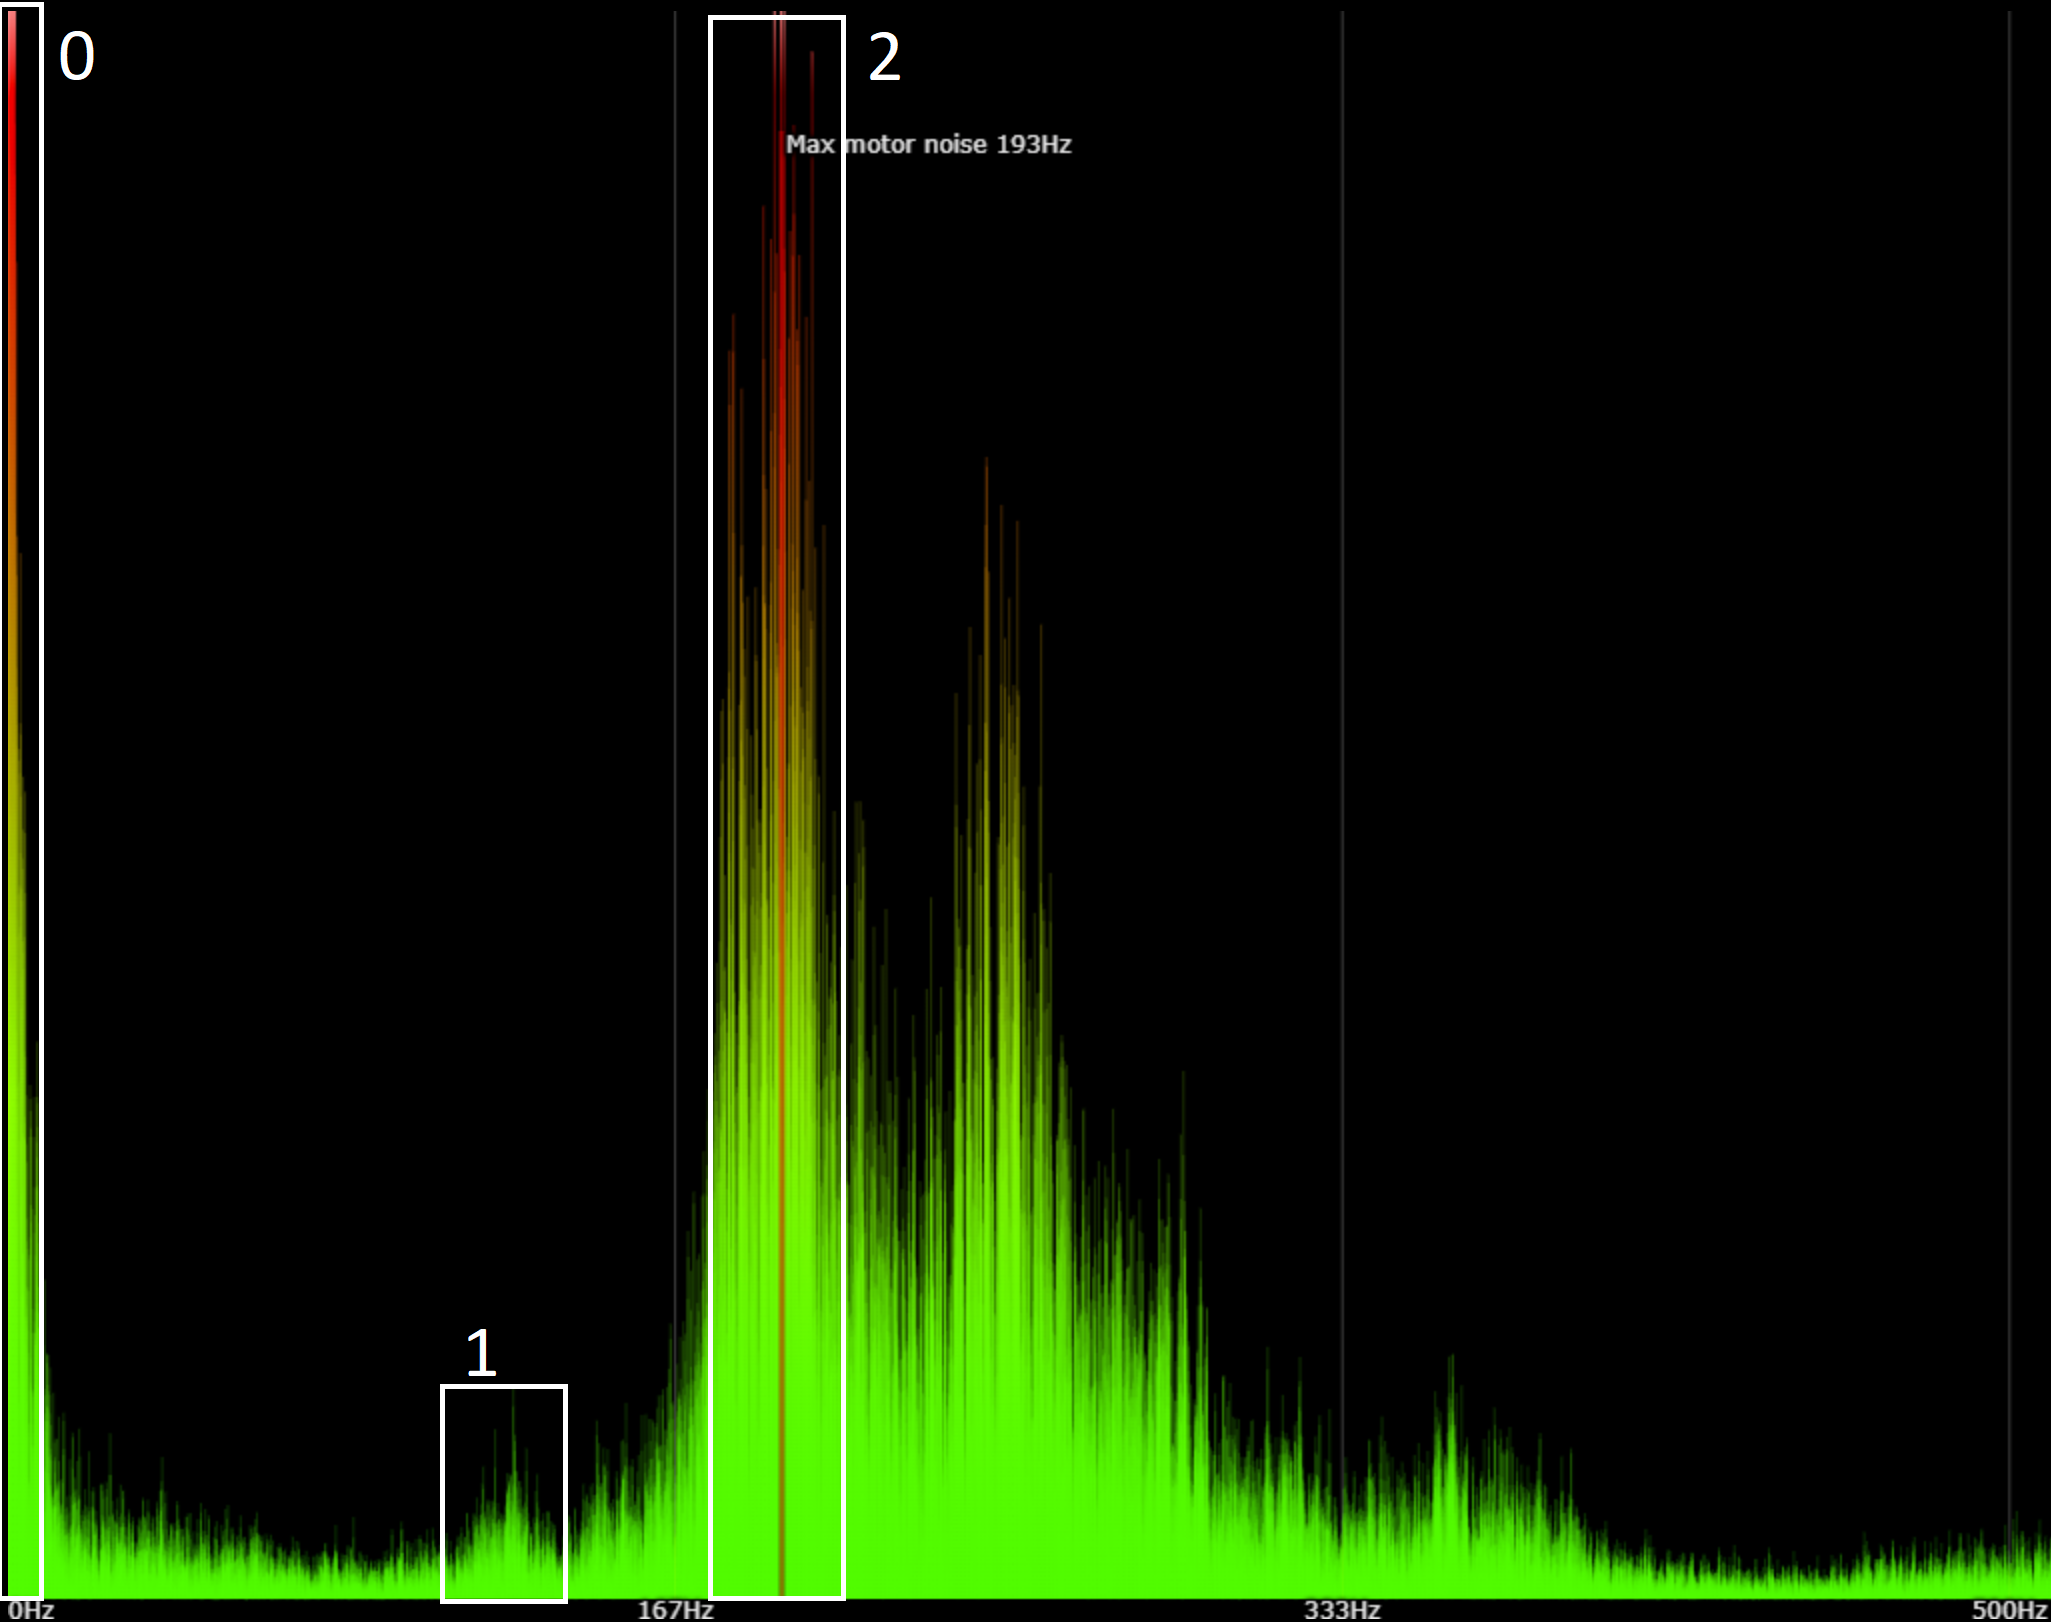
\includegraphics[width=\textwidth]{Img/Diagramm_vor_Filterung_PitchAchse}
                \caption{Signal vor der Filterung}
                \label{VorFilterung}
            \end{subfigure}
            \hfill
            \begin{subfigure}[b]{0.49\textwidth}
                \centering
                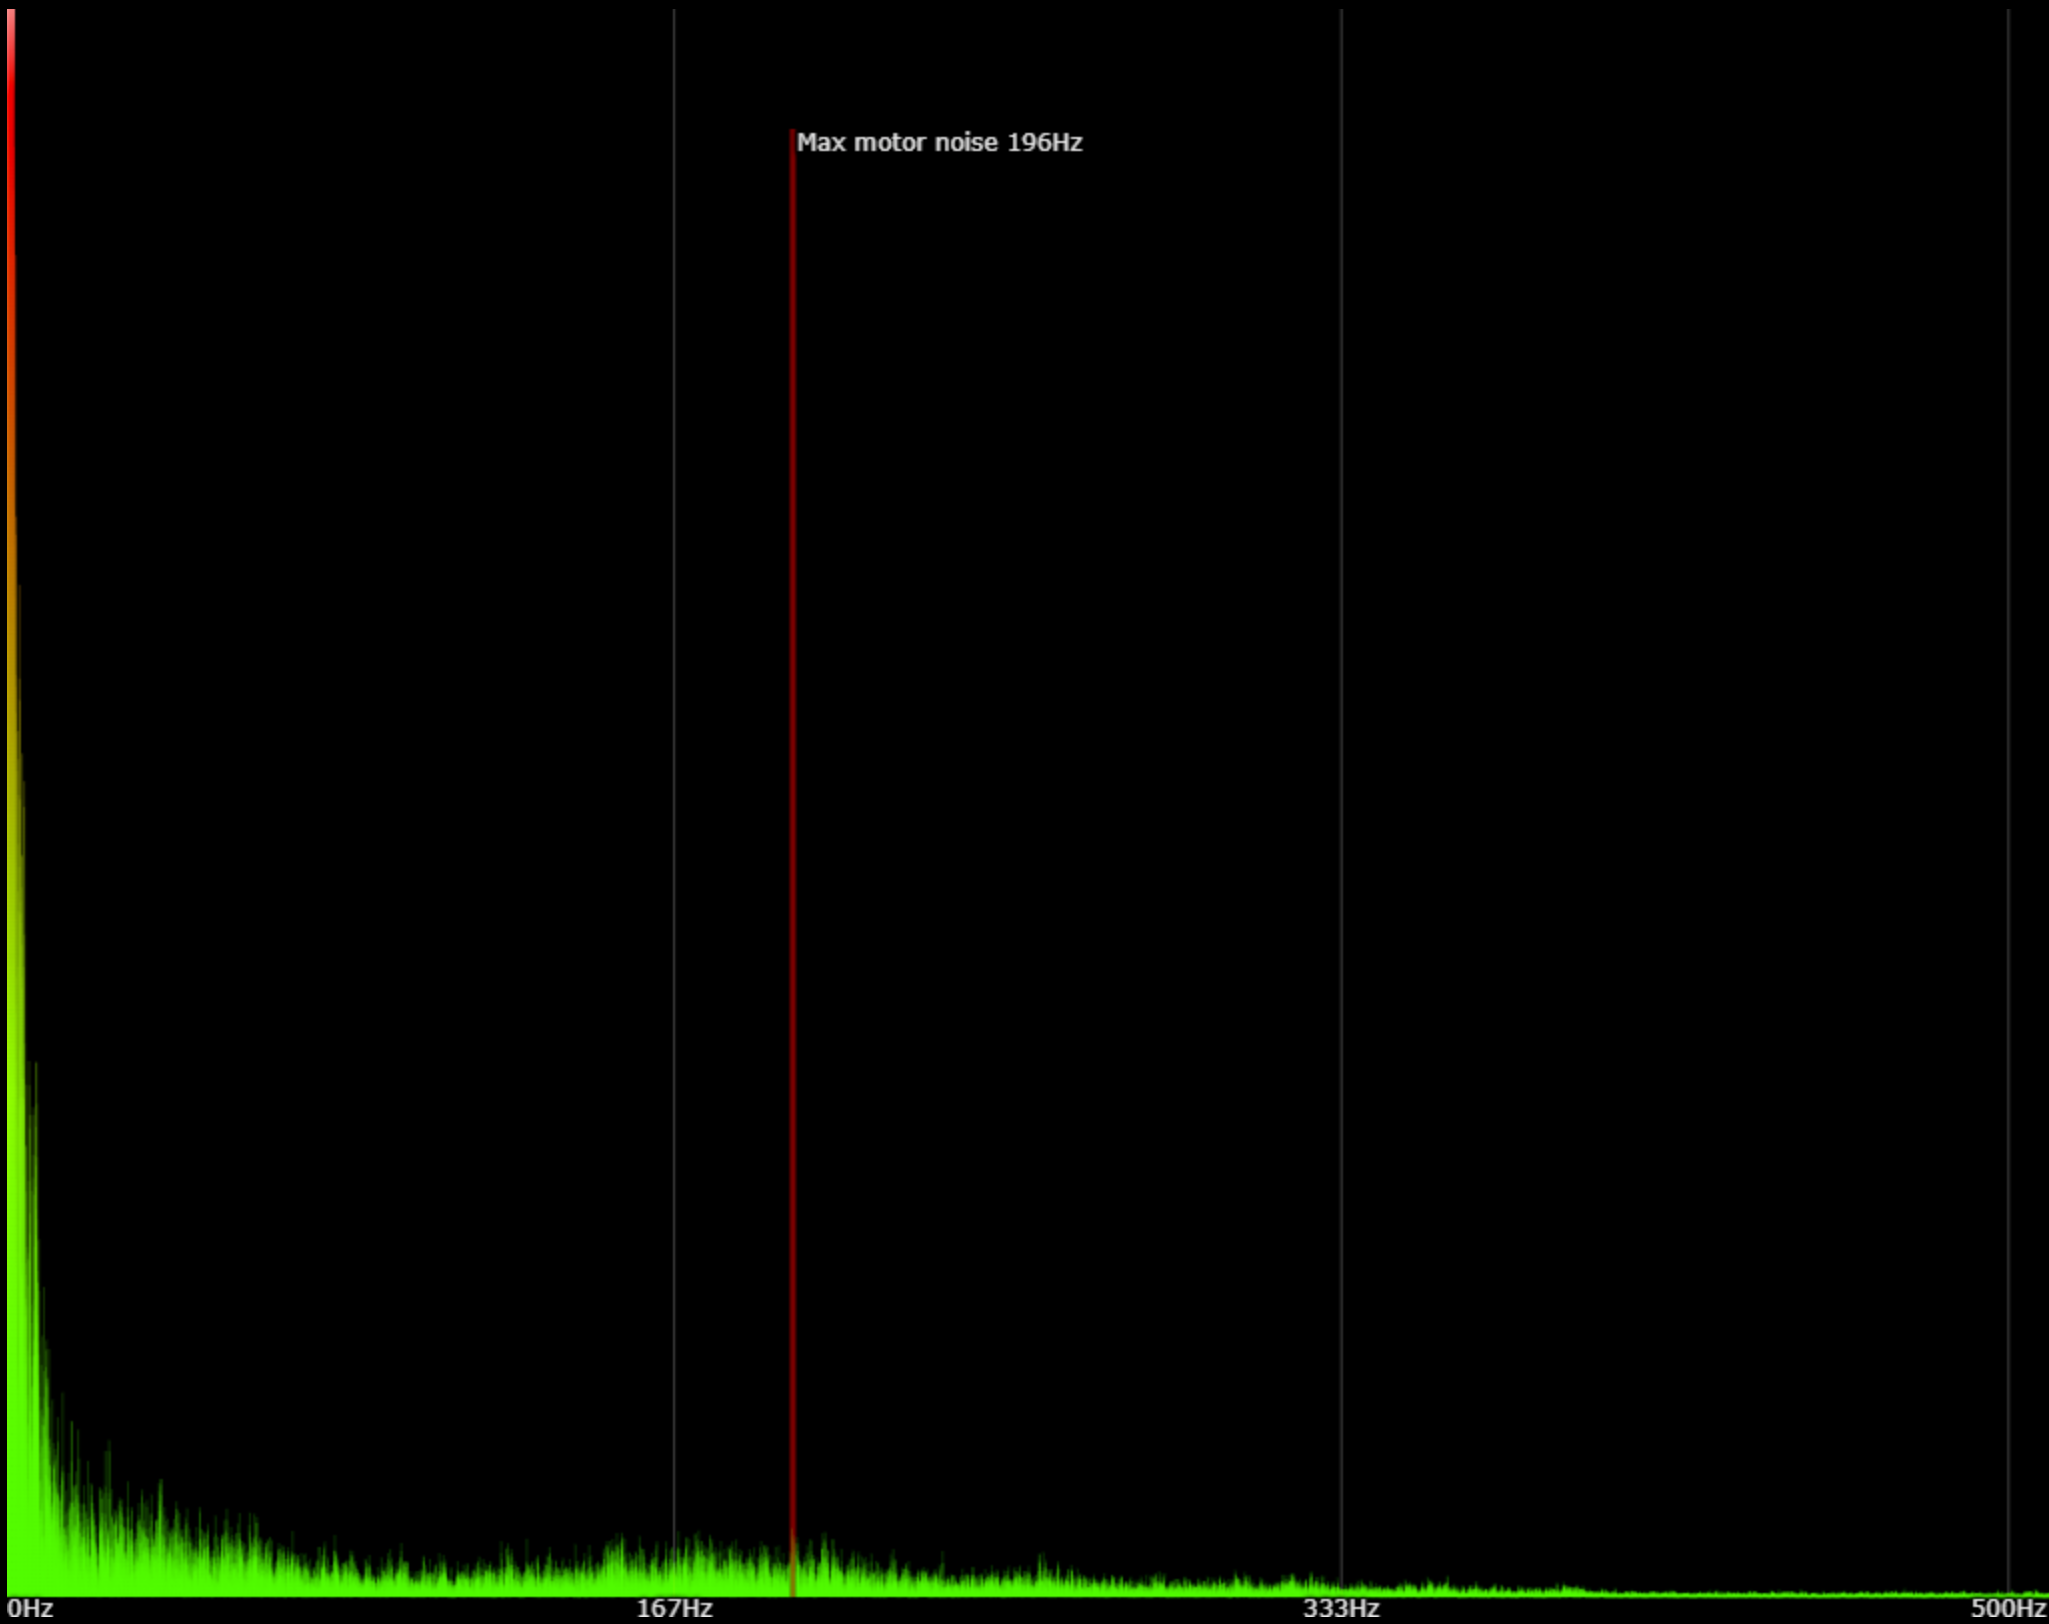
\includegraphics[width=\textwidth]{Img/Diagramm_nach_Filterung_PitchAchse}
                \caption{Signal nach der Filterung}
                \label{NachFilterung}
            \end{subfigure}
               \caption{Auswirkungen einer korrekten Filterung}
               \label{AuswirkungenFilterung}
       \end{figure}

       Für die folgende Betrachtung der Diagramme werden keine Werte benötigt. Das Experiment soll nur
       einen Überblick über die Möglichkeiten einer korrekten Filterung darlegen und grafisch zeigen,
       wie sich dies im Signal bemerkbar macht. Auf der horizontalen Achse der Abbildung~\ref*{VorFilterung}
       und~\ref*{NachFilterung} ist jeweils die Frequenz der Vibration bzw. Bewegung dargestellt.
       Die vertikale Achse beschreibt die Amplitude und somit die Intensität. \\
       \\
       Abbildung~\ref*{VorFilterung} zeigt das ungefilterte Signal des Gyroskops, welches ein hohes Maß an Rauschen aufweist.
       Neben einem hohen Grundrauschen lassen sich zwei Effekte besonders gut erkennen. Zum einen das
       sogenannte „prop wash“, welches in Abbildung a durch die Zahl 1 gekennzeichnet ist, zum anderen
       die Resonanzfrequenz des Systems, welche sich bei ungefähr \qty{200}{\Hz} mit einer hohen Amplitude zeigt
       und mit der Nummer 2 gekennzeichnet ist. \\
       \\
       In Abbildung~\ref*{NachFilterung} lässt sich das identische, jedoch gefilterte Signal des Gyroskops erkennen. Dieses
       Signal wird im weiteren Verlauf dem PID-Loop als „Ist-Wert“ zur Verfügung gestellt. In Abbildung~\ref*{NachFilterung} lässt
       sich eindeutig erkennen, dass ein Großteil der Frequenzen herausgefiltert wurde. Jedoch noch
       immer ein geringfügiges Rauschen im Bereich von \qty{200}{\Hz} vorhanden ist. Da die Amplitude dieser Störungen
       jedoch im Vergleich zu den eigentlichen Bewegungen der Drohne minimal ist, kann diese vernachlässigt werden. \\
       \\
       Frequenzen unterhalb von \qty{100}{\Hz} werden im Normalfall nicht gefiltert bzw. gedämpft, da diese Frequenzen
       das Resultat einer tatsächlichen Bewegung der Drohne darstellen. Dies kann sowohl in Abbildung~\ref*{VorFilterung} als auch
       in Abbildung~\ref*{NachFilterung} beobachtet werden. Die betroffenen Bereiche sind mit der Zahl 0 in beiden Abbildungen markiert.
    \newpage 
    \subsection[Rahmen]{Rahmen}
        Der Rahmen, oft auch als „Frame“ bezeichnet, bildet das Grundgerüst einer jeden FPV-Drohne.
        Er besteht aus einem leichten, aber robusten Material wie Kohlefaser und nimmt erheblichen
        Einfluss auf das Flugverhalten der Drohne. Die Größe des Rahmens beeinflusst nicht nur das
        Erscheinungsbild, sondern die gesamte Konstruktion der FPV-Drohne. Aus diesem Grund ist es
        unerlässlich, dass die Größe des Rahmens sorgfältig geplant und ausgewählt wird. Die Wahl
        des Rahmens bestimmt im weiteren Verlauf die Auswahl und Anordnung der weiteren Komponenten
        wie Motoren, Propeller und Akku, welche auf den Rahmen abgestimmt werden müssen, um ein
        optimales Flugverhalten zu gewährleisten. \\
        \\
        Die Größe eines FPV-Drohnenrahmens wird in der Regel in Zoll (inch) angegeben und bezieht
        sich auf den Durchmesser der Propeller, welche an diesem Rahmen maximal verwendet werden
        können. Eine weitere wichtige Kenngröße ist die Dicke des Rahmens. Ein dicker Rahmen sorgt
        für eine höhere Steifigkeit, was zu einem präziseren und stabileren Flug führt. Allerdings
        erhöht dieser auch das Gewicht und könnte so das Flugverhalten und die Manövrierfähigkeit
        beeinträchtigen. Ein dünner Rahmen ist leichter, bietet dadurch eine längere Akkulaufzeit
        und höhere Manövrierfähigkeit, kann allerdings auch anfälliger für Beschädigungen und durch
        die geringere Steifigkeit weniger stabil im Flug sein. \\
        \\
        Zusätzlich haben die Dicke und Größe des Rahmens Einfluss auf die Weiterleitung von
        Vibrationen, welche durch die Motoren entstehen und sich in den Rahmen fortbewegen. Starke
        Vibrationen können zu Fehlern im PID-Loop führen, da Messwerte des Gyroskops und anderer
        Sensoren beeinträchtigt und verfälscht werden. Neben den Flugeigenschaften leidet auch die
        Videoqualität unter Vibrationen, welche die Kamera erreichen. Diese Vibrationen können durch
        einen dickeren Rahmen minimiert werden. Auch die Größe des Rahmens hat Einfluss auf die
        Vibrationen, so erfährt beispielsweise ein 7\dq Rahmen deutlich mehr Vibrationen bei gleicher
        Dicke als ein 5\dq Rahmen, da die Arme des 7\dq Rahmens länger sind, was zu einer reduzierten
        Steifigkeit und somit mehr Vibrationen führt. Diesem Effekt kann durch eine passende Filterung
        entgegengewirkt werden.

    \subsection[Propeller]{Propeller}
        Die Propeller haben direkten Einfluss auf das Flugverhalten und so indirekt auch Einfluss auf
        die Videoqualität. Sie werden durch die Motoren auf enorme Geschwindigkeiten beschleunigt und
        erzeugen so den Auftrieb für den Flug. Propeller zeichnen sich durch drei wichtige Kenndaten
        aus. Den Durchmesser und die Steigung, welche meist in Zoll angegeben werden und die Anzahl
        der Propellerflügel. All diese Kenndaten haben einen enormen Einfluss auf sämtliche Aspekte der
        FPV-Drohne, wie beispielsweise das Flugverhalten oder die Akkulaufzeit. \\
        \\
        Der Durchmesser gibt an, wie groß der Propeller ist und beeinflusst direkt die Menge an Luft,
        die er in einer bestimmten Zeit bewegen kann. Die Steigung kann symbolisch mit der Steigung
        eines Gewindes veranschaulicht werden. Je höher die Steigung ist, desto tiefer dringt die Schraube
        pro Umdrehung in das Material vor.
    \newpage
        Dies benötigt jedoch mehr Kraft beziehungsweise Energie. Gleiches
        gilt für die Steigung eines Propellers. Dieser kann durch eine höhere Steigung bei gleichbleibender
        Anzahl der Umdrehung mehr Luft befördern, benötigt jedoch ein höheres Drehmoment bzw. mehr Energie
        durch den Motor. Die Anzahl der Flügel nimmt besonders Einfluss auf die übertragbare Leistung und
        die Effizienz. Da durch jeden Flügel eines Propellers die von Luft durchströmte Fläche erhöht wird,
        kann ein Propeller mit mehr Flügeln bei gleichbleibendem Durchmesser mehr Luft befördern als einer
        mit weniger Flügeln. Da diese sich jedoch gegenseitig negativ beeinflussen und Turbulenzen erzeugen,
        sinkt die Effizienz, was in einem höheren Energieverbrauch resultiert.  \\
        \\
        Ein weiterer Aspekt, welche beachtet werden muss, ist die mechanische Integrität. Falls ein Propeller
        beispielsweise durch einen Absturz beschädigt oder verbogen worden ist, sollte dieser vor dem nächsten
        Flug entfernt und durch einen neuen ersetzt werden. Andernfalls kann es aufgrund der enormen
        Rotationsgeschwindigkeiten des Propellers, welcher möglicherweise durch den Defekt nicht mehr exakt ausgewuchtet
        ist, zu Vibrationen kommen. Aufgrund der Intensität diese kann der FC sie unter Umständen nicht korrekt
        filtern, was in unkontrollierten Bewegungen der Drohne resultieren würde. \\
        \\
        Die Geschwindigkeit des Propellers wird durch zwei Faktoren beeinflusst. Zum einen durch die Spannung,
        welche am Motor anliegt und zum anderen durch den $kv$-Wert (Umdrehungen pro Minute pro Volt,
        $\frac{1}{\si{\minute}\cdot \si{\volt}}$), den dieser Motor besitzt. In der folgenden Rechnung wird
        beispielhaft und vereinfacht die Umdrehungszahl eines Motors und die Geschwindigkeit des Propellers
        für eine 6$s$ System mit einem Motor mit 1950$kv$ und einem 5\dq Propeller berechnet. 6$s$ gibt hierbei
        die Anzahl an Zellen und somit die Höhe der Spannung an. Es wird zur Vereinfachung davon ausgegangen,
        dass die Spannung einer Zelle auch unter Last konstant bei \qty{3,7}{\volt} liegt.
    
        \begin{equation}
            n=\frac{s\cdot\qty{3,7}{\volt}\cdot kv}{60}
        \end{equation}

        Werden für $s$ und $kv$ die Werte aus dem Beispiel eingesetzt, erhält man
        $n=\num{721,5} \frac{1}{\si{\second}} = \num{43290} \frac{1}{\si{\minute}}$. Um nun die Geschwindigkeit
        an der Spitze eines Propellerflügels zu berechnen, kann folgende Formel verwendet werden.
        
        \begin{equation}
            v=D\cdot \pi \cdot n
        \end{equation}

        Nach Einsetzen des Durchmessers und der berechneten Umdrehungsanzahl ergibt sich eine Geschwindigkeit
        von $v\approx \qty{287,87}{\meter\per\second} \approx \qty{1036}{\kilo\meter\per\hour}$ an der Spitze
        des Propellerflügels. Diese enormen Geschwindigkeiten werden in der Realität aufgrund von Luftwiderstand,
        Verlustleistungen und dem begrenzten Strom des Akkus nicht erreicht. Sie zeigt jedoch den Bereich, in dem
        sich die Geschwindigkeit des Propellers bewegt und lässt erahnen, welche Folgen eine Unwucht hätte.